\documentclass[border=10pt, tikz]{standalone}

\usetikzlibrary{
    positioning,
    arrows.meta,
    calc,
    decorations.markings,
    fit,
    backgrounds,
    shapes.geometric,
    fadings,
    patterns
}

\usepackage{amsmath, amssymb}
\usepackage{xcolor}

% ============================================
% BIORENDER-INSPIRED SOFT PALETTE
% ============================================
% Tissue/organ colors
\definecolor{tissue}{HTML}{F5E8E0}
\definecolor{tissuerim}{HTML}{D8B4A8}
\definecolor{stroma}{HTML}{EAD9C4}
\definecolor{stromadark}{HTML}{C4A87E}

% Cell colors - soft pastels
\definecolor{epithelial}{HTML}{A8D5BA}
\definecolor{epithelialdark}{HTML}{5A9A70}
\definecolor{immune}{HTML}{B8D4E8}
\definecolor{immunedark}{HTML}{5A8CB0}
\definecolor{fibroblast}{HTML}{E8C8D8}
\definecolor{fibroblastdark}{HTML}{B87A98}
\definecolor{macrophage}{HTML}{F5D89A}
\definecolor{macrophagedark}{HTML}{C8A040}

% Receiver/target
\definecolor{recv}{HTML}{E85A5A}
\definecolor{recvdark}{HTML}{A03030}
\definecolor{recvglow}{HTML}{FFB8B8}

% Stage progression colors
\definecolor{normal}{HTML}{B8E0D2}
\definecolor{normaldark}{HTML}{5AA888}
\definecolor{aah}{HTML}{C5E8B0}
\definecolor{aahdark}{HTML}{78B850}
\definecolor{ais}{HTML}{F5E6A0}
\definecolor{aisdark}{HTML}{C8B040}
\definecolor{luad}{HTML}{F5B8A0}
\definecolor{luaddark}{HTML}{C87050}

% Accent for flow
\definecolor{accent}{HTML}{E07B54}
\definecolor{accentglow}{HTML}{FADDD1}

% UI colors
\definecolor{boxbg}{HTML}{FAFCFD}
\definecolor{boxline}{HTML}{E0E4E8}
\definecolor{textmain}{HTML}{2C3E50}
\definecolor{textsub}{HTML}{7F8C9A}

% ============================================
% BIORENDER-STYLE DEFINITIONS
% ============================================

\tikzset{
    % Soft box for encoder
    softbox/.style={
        rectangle,
        rounded corners=4pt,
        fill=#1!15,
        draw=#1!50,
        line width=0.5pt,
        minimum height=10mm,
        minimum width=26mm,
        font=\fontsize{8}{9}\selectfont\sffamily,
        text=textmain
    },
    % Panel
    panel/.style={
        rectangle,
        rounded corners=6pt,
        fill=white,
        draw=boxline,
        line width=0.5pt
    },
    % Flow trajectory
    flowtraj/.style={
        line width=2pt,
        draw=accent,
        postaction={decorate, decoration={markings,
            mark=at position 0.3 with {\arrow[accent, scale=0.8]{Stealth}},
            mark=at position 0.6 with {\arrow[accent, scale=0.8]{Stealth}}
        }}
    },
    % Attention line
    attnline/.style={
        -{Stealth[length=2mm, width=1.5mm]},
        line width=0.6pt,
        draw=accent,
        opacity=0.5
    },
    % Labels
    title/.style={font=\fontsize{11}{12}\selectfont\bfseries\sffamily, text=textmain},
    subtitle/.style={font=\fontsize{7.5}{8.5}\selectfont\sffamily, text=textsub},
    annot/.style={font=\fontsize{6.5}{7.5}\selectfont\sffamily, text=textsub},
    celltype/.style={font=\fontsize{5.5}{6.5}\selectfont\sffamily, text=textmain},
    math/.style={font=\fontsize{7.5}{8.5}\selectfont, text=textsub},
    % Arrows
    arr/.style={-{Stealth[length=2.2mm, width=1.6mm]}, line width=0.6pt, draw=textsub},
    arraccent/.style={-{Stealth[length=2.8mm, width=2mm]}, line width=0.8pt, draw=accent},
    % Dashed ring for spatial zones
    spatialring/.style={
        draw=#1,
        line width=0.6pt,
        dashed,
        dash pattern=on 3pt off 2pt
    },
}

% ============================================
% CELL DRAWING MACROS
% ============================================
% Draw cell with nucleus: \cell{x}{y}{size}{fillcolor}{darkcolor}
\newcommand{\cell}[5]{%
    \fill[#4, draw=#5, line width=0.4pt] (#1, #2) circle (#3);%
    \fill[#5!60] (#1, #2) circle ({#3*0.35});%
}
% Draw stage cell: \stagecell{x}{y}{color}
\newcommand{\stagecellcmd}[3]{%
    \fill[#3, draw=#3dark, line width=0.4pt] (#1, #2) circle (2.2mm);%
    \fill[#3dark!50] (#1, #2) circle (0.8mm);%
}
% Draw receiver cell with glow: \recvcell{x}{y}{size}
\newcommand{\recvcellcmd}[3]{%
    \fill[recvglow] (#1, #2) circle ({#3*1.4});%
    \fill[recv, draw=recvdark, line width=0.7pt] (#1, #2) circle (#3);%
    \fill[recvdark!70] (#1, #2) circle ({#3*0.25});%
}
% Draw stroma/tissue background: \stromabg{x}{y}{w}{h}
\newcommand{\stromabg}[4]{%
    \fill[stroma, rounded corners=4mm, draw=stromadark, line width=0.6pt]
        ({#1-#3/2}, {#2-#4/2}) rectangle ({#1+#3/2}, {#2+#4/2});%
}
% Draw tissue section: \tissuesection{x}{y}{w}{h}
\newcommand{\tissuesection}[4]{%
    \fill[tissue, rounded corners=6mm, draw=tissuerim, line width=0.8pt]
        ({#1-#3/2}, {#2-#4/2}) rectangle ({#1+#3/2}, {#2+#4/2});%
}

\begin{document}
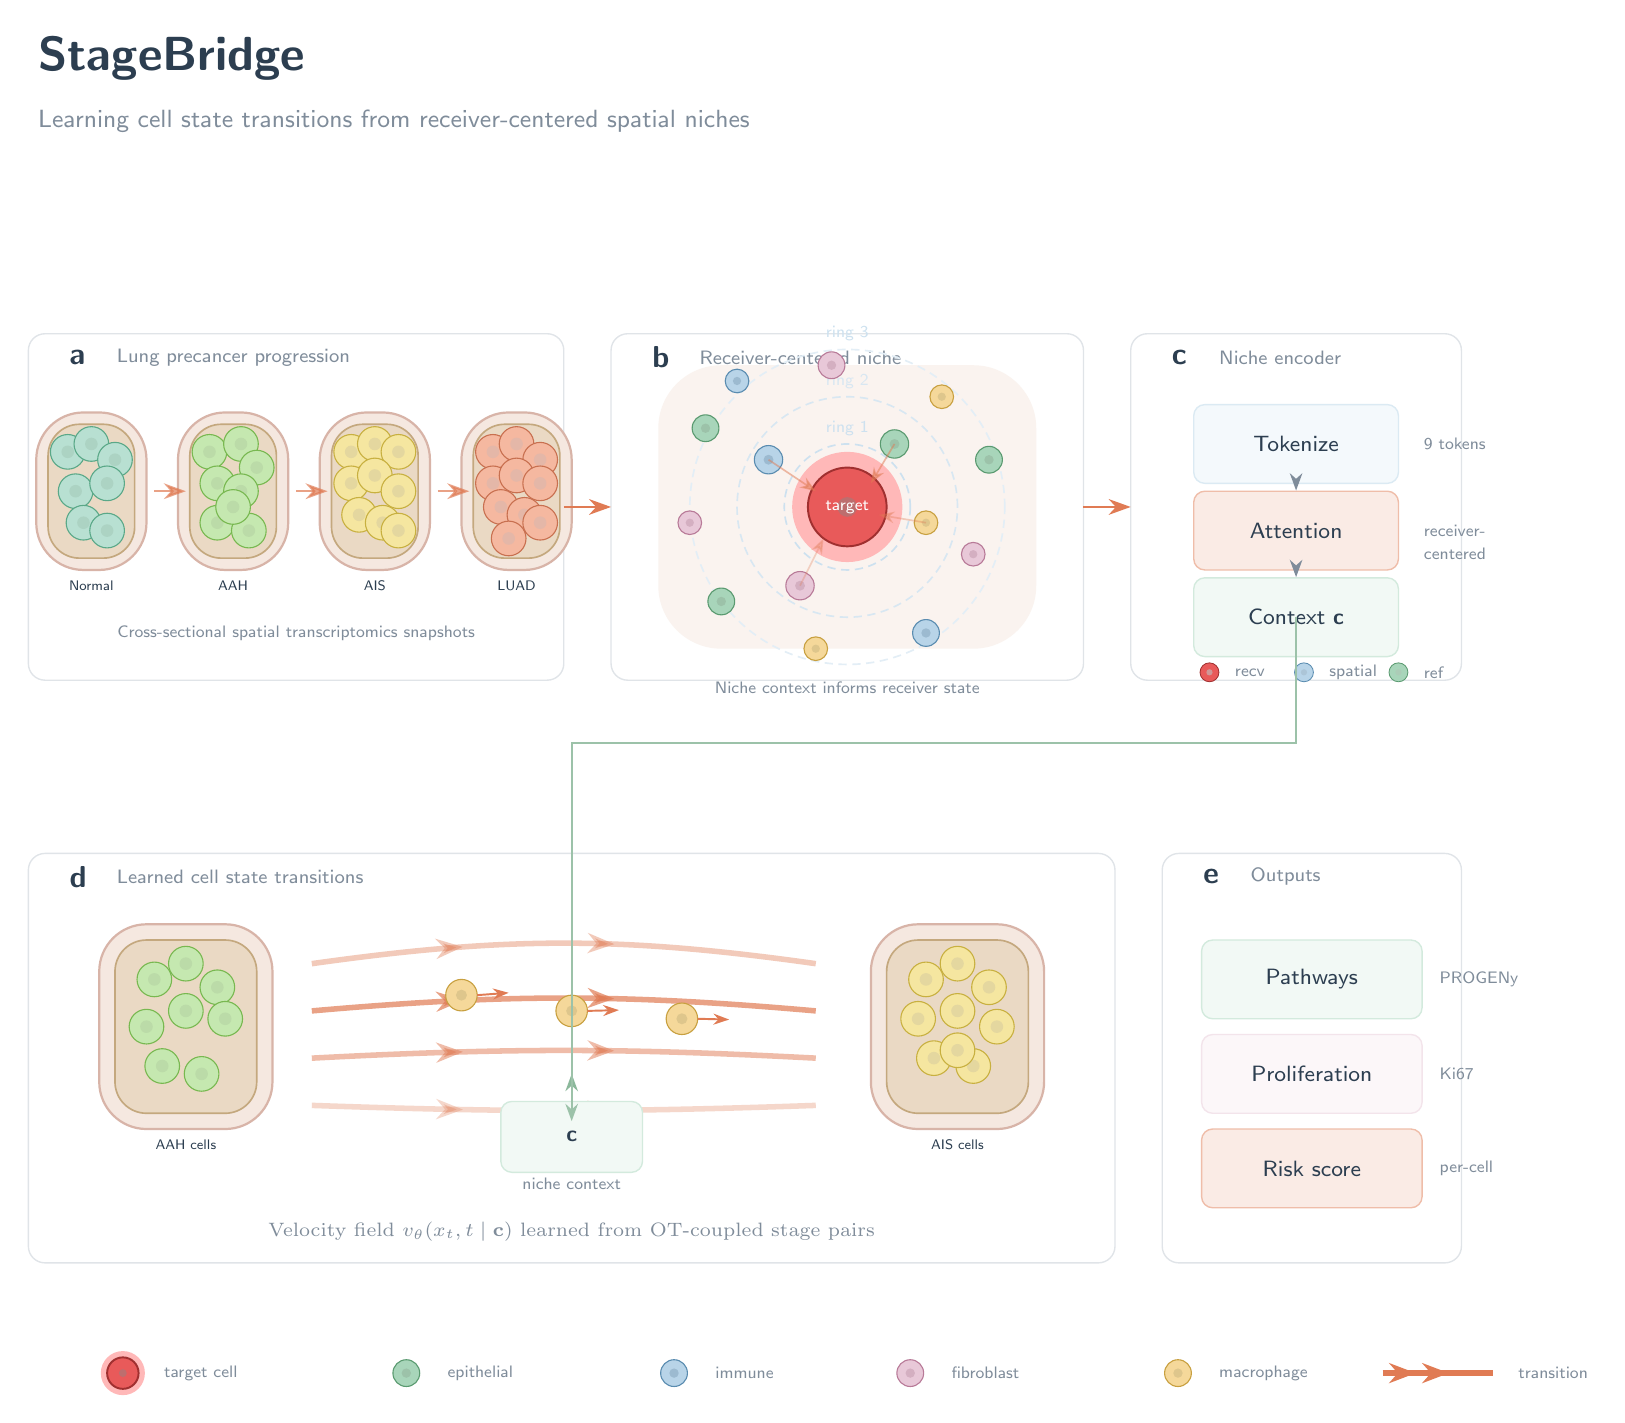
\begin{tikzpicture}[x=1mm, y=1mm]

% ============================================
% HEADER
% ============================================
\node[font=\fontsize{16}{18}\selectfont\bfseries\sffamily, text=textmain, anchor=west]
    at (0, 92) {StageBridge};
\node[font=\fontsize{9}{10}\selectfont\sffamily, text=textsub, anchor=west]
    at (0, 84) {Learning cell state transitions from receiver-centered spatial niches};

% ============================================
% a) LUNG PRECANCER PROGRESSION
% ============================================
\begin{scope}[shift={(0, 35)}]
    \node[panel, minimum width=68mm, minimum height=44mm] at (34, 0) {};
    \node[title, anchor=west] at (4, 19) {a};
    \node[subtitle, anchor=west] at (10, 19) {Lung precancer progression};

    % Normal alveoli - tissue section with cells
    \begin{scope}[shift={(8, 2)}]
        \tissuesection{0}{0}{14}{20}
        \stromabg{0}{0}{11}{17}
        \stagecellcmd{-3}{5}{normal}
        \stagecellcmd{0}{6}{normal}
        \stagecellcmd{3}{4}{normal}
        \stagecellcmd{-2}{0}{normal}
        \stagecellcmd{2}{1}{normal}
        \stagecellcmd{-1}{-4}{normal}
        \stagecellcmd{2}{-5}{normal}
        \node[celltype] at (0, -12) {Normal};
    \end{scope}

    % AAH - more cells, slight dysplasia
    \begin{scope}[shift={(26, 2)}]
        \tissuesection{0}{0}{14}{20}
        \stromabg{0}{0}{11}{17}
        \stagecellcmd{-3}{5}{aah}
        \stagecellcmd{1}{6}{aah}
        \stagecellcmd{3}{3}{aah}
        \stagecellcmd{-2}{1}{aah}
        \stagecellcmd{1}{0}{aah}
        \stagecellcmd{-2}{-4}{aah}
        \stagecellcmd{2}{-5}{aah}
        \stagecellcmd{0}{-2}{aah}
        \node[celltype] at (0, -12) {AAH};
    \end{scope}

    % AIS - more crowded
    \begin{scope}[shift={(44, 2)}]
        \tissuesection{0}{0}{14}{20}
        \stromabg{0}{0}{11}{17}
        \stagecellcmd{-3}{5}{ais}
        \stagecellcmd{0}{6}{ais}
        \stagecellcmd{3}{5}{ais}
        \stagecellcmd{-3}{1}{ais}
        \stagecellcmd{0}{2}{ais}
        \stagecellcmd{3}{0}{ais}
        \stagecellcmd{-2}{-3}{ais}
        \stagecellcmd{1}{-4}{ais}
        \stagecellcmd{3}{-5}{ais}
        \node[celltype] at (0, -12) {AIS};
    \end{scope}

    % LUAD - most crowded, invasive
    \begin{scope}[shift={(62, 2)}]
        \tissuesection{0}{0}{14}{20}
        \stromabg{0}{0}{11}{17}
        \stagecellcmd{-3}{5}{luad}
        \stagecellcmd{0}{6}{luad}
        \stagecellcmd{3}{4}{luad}
        \stagecellcmd{-3}{1}{luad}
        \stagecellcmd{0}{2}{luad}
        \stagecellcmd{3}{1}{luad}
        \stagecellcmd{-2}{-2}{luad}
        \stagecellcmd{1}{-3}{luad}
        \stagecellcmd{3}{-4}{luad}
        \stagecellcmd{-1}{-6}{luad}
        \node[celltype] at (0, -12) {LUAD};
    \end{scope}

    % Progression arrows
    \draw[arraccent, opacity=0.7] (16, 2) -- (20, 2);
    \draw[arraccent, opacity=0.7] (34, 2) -- (38, 2);
    \draw[arraccent, opacity=0.7] (52, 2) -- (56, 2);

    \node[annot] at (34, -16) {Cross-sectional spatial transcriptomics snapshots};
\end{scope}

% ============================================
% b) RECEIVER-CENTERED NICHE (hero visual)
% ============================================
\begin{scope}[shift={(74, 35)}]
    \node[panel, minimum width=60mm, minimum height=44mm] at (30, 0) {};
    \node[title, anchor=west] at (4, 19) {b};
    \node[subtitle, anchor=west] at (10, 19) {Receiver-centered niche};

    % Tissue background for the niche
    \fill[tissue!50, rounded corners=8mm] (6, -18) rectangle (54, 18);

    % Spatial rings (distance zones)
    \draw[spatialring=immune!40] (30, 0) circle (20mm);
    \draw[spatialring=immune!55] (30, 0) circle (14mm);
    \draw[spatialring=immune!70] (30, 0) circle (8mm);

    % Ring labels
    \node[annot, immune!70] at (30, 22) {ring 3};
    \node[annot, immune!55] at (30, 16) {ring 2};
    \node[annot, immune!70] at (30, 10) {ring 1};

    % Diverse neighbor cells (outer ring)
    \cell{12}{10}{1.7mm}{epithelial}{epithelialdark}
    \cell{16}{16}{1.5mm}{immune}{immunedark}
    \cell{28}{18}{1.7mm}{fibroblast}{fibroblastdark}
    \cell{42}{14}{1.5mm}{macrophage}{macrophagedark}
    \cell{48}{6}{1.7mm}{epithelial}{epithelialdark}
    \cell{46}{-6}{1.5mm}{fibroblast}{fibroblastdark}
    \cell{40}{-16}{1.7mm}{immune}{immunedark}
    \cell{26}{-18}{1.5mm}{macrophage}{macrophagedark}
    \cell{14}{-12}{1.7mm}{epithelial}{epithelialdark}
    \cell{10}{-2}{1.5mm}{fibroblast}{fibroblastdark}

    % Inner ring cells (closer to receiver)
    \cell{20}{6}{1.8mm}{immune}{immunedark}
    \cell{36}{8}{1.8mm}{epithelial}{epithelialdark}
    \cell{40}{-2}{1.5mm}{macrophage}{macrophagedark}
    \cell{24}{-10}{1.8mm}{fibroblast}{fibroblastdark}

    % Receiver cell (with glow effect) - drawn last to be on top
    \recvcellcmd{30}{0}{5mm}
    \node[font=\fontsize{6}{7}\selectfont\sffamily, text=white] at (30, 0) {target};

    % Attention lines from inner neighbors
    \draw[attnline] (20, 6) -- (26, 2);
    \draw[attnline] (36, 8) -- (33, 3);
    \draw[attnline, opacity=0.35] (40, -2) -- (34, -1);
    \draw[attnline, opacity=0.3] (24, -10) -- (27, -4);

    \node[annot] at (30, -23) {Niche context informs receiver state};
\end{scope}

% ============================================
% c) NICHE ENCODER
% ============================================
\begin{scope}[shift={(140, 35)}]
    \node[panel, minimum width=42mm, minimum height=44mm] at (21, 0) {};
    \node[title, anchor=west] at (4, 19) {c};
    \node[subtitle, anchor=west] at (10, 19) {Niche encoder};

    % Encoder stack with soft boxes
    \node[softbox=immune] (tok) at (21, 8) {Tokenize};
    \node[annot, anchor=west] at (36, 8) {9 tokens};

    \node[softbox=accent] (attn) at (21, -3) {Attention};
    \node[annot, anchor=west] at (36, -3) {receiver-};
    \node[annot, anchor=west] at (36, -6) {centered};

    \node[softbox=epithelial] (ctx) at (21, -14) {Context \textbf{c}};

    \draw[arr] (tok) -- (attn);
    \draw[arr] (attn) -- (ctx);

    % Token types mini-legend
    \fill[recv, draw=recvdark, line width=0.3pt] (10, -21) circle (1.2mm);
    \fill[recvdark!50] (10, -21) circle (0.4mm);
    \node[annot, anchor=west] at (12, -21) {recv};

    \fill[immune, draw=immunedark, line width=0.3pt] (22, -21) circle (1.2mm);
    \fill[immunedark!50] (22, -21) circle (0.4mm);
    \node[annot, anchor=west] at (24, -21) {spatial};

    \fill[epithelial, draw=epithelialdark, line width=0.3pt] (34, -21) circle (1.2mm);
    \fill[epithelialdark!50] (34, -21) circle (0.4mm);
    \node[annot, anchor=west] at (36, -21) {ref};
\end{scope}

% Arrows between top panels
\draw[arraccent] (68, 35) -- (74, 35);
\draw[arraccent] (134, 35) -- (140, 35);

% ============================================
% d) LEARNED CELL STATE TRANSITIONS
% ============================================
\begin{scope}[shift={(0, -35)}]
    \node[panel, minimum width=138mm, minimum height=52mm] at (69, 0) {};
    \node[title, anchor=west] at (4, 23) {d};
    \node[subtitle, anchor=west] at (10, 23) {Learned cell state transitions};

    % Source distribution (AAH cells) with tissue
    \begin{scope}[shift={(20, 4)}]
        \tissuesection{0}{0}{22}{26}
        \stromabg{0}{0}{18}{22}
        \stagecellcmd{-4}{6}{aah}
        \stagecellcmd{0}{8}{aah}
        \stagecellcmd{4}{5}{aah}
        \stagecellcmd{-5}{0}{aah}
        \stagecellcmd{0}{2}{aah}
        \stagecellcmd{5}{1}{aah}
        \stagecellcmd{-3}{-5}{aah}
        \stagecellcmd{2}{-6}{aah}
        \node[celltype] at (0, -15) {AAH cells};
    \end{scope}

    % Target distribution (AIS cells) with tissue
    \begin{scope}[shift={(118, 4)}]
        \tissuesection{0}{0}{22}{26}
        \stromabg{0}{0}{18}{22}
        \stagecellcmd{-4}{6}{ais}
        \stagecellcmd{0}{8}{ais}
        \stagecellcmd{4}{5}{ais}
        \stagecellcmd{-5}{1}{ais}
        \stagecellcmd{0}{2}{ais}
        \stagecellcmd{5}{0}{ais}
        \stagecellcmd{-3}{-4}{ais}
        \stagecellcmd{2}{-5}{ais}
        \stagecellcmd{0}{-3}{ais}
        \node[celltype] at (0, -15) {AIS cells};
    \end{scope}

    % Flow trajectories (multiple paths showing distribution)
    \draw[flowtraj, opacity=0.4] (36, 12) to[out=8, in=172] (100, 12);
    \draw[flowtraj, opacity=0.7] (36, 6) to[out=5, in=175] (100, 6);
    \draw[flowtraj, opacity=0.5] (36, 0) to[out=3, in=177] (100, 0);
    \draw[flowtraj, opacity=0.3] (36, -6) to[out=-2, in=182] (100, -6);

    % Intermediate states with velocity vectors - cells along trajectory
    \cell{55}{8}{2mm}{macrophage}{macrophagedark}
    \cell{69}{6}{2mm}{macrophage}{macrophagedark}
    \cell{83}{5}{2mm}{macrophage}{macrophagedark}

    \draw[-{Stealth[length=2mm, width=1.4mm]}, accent, line width=0.7pt] (57, 8) -- ++(4, 0.3);
    \draw[-{Stealth[length=2mm, width=1.4mm]}, accent, line width=0.7pt] (71, 6) -- ++(4, 0.1);
    \draw[-{Stealth[length=2mm, width=1.4mm]}, accent, line width=0.7pt] (85, 5) -- ++(4, -0.1);

    % Context conditioning
    \node[softbox=epithelial, minimum width=18mm, minimum height=9mm] (ctxd) at (69, -10) {\textbf{c}};
    \draw[arr, draw=epithelialdark!70] (ctxd) -- (69, -2);
    \node[annot] at (69, -16) {niche context};

    % Velocity field equation
    \node[math] at (69, -22) {Velocity field $v_\theta(x_t, t \mid \mathbf{c})$ learned from OT-coupled stage pairs};
\end{scope}

% Context connection from encoder
\draw[arr, draw=epithelialdark!60] (161, 21) -- (161, 5) -| (69, -43);

% ============================================
% e) BIOLOGICAL OUTPUTS
% ============================================
\begin{scope}[shift={(144, -35)}]
    \node[panel, minimum width=38mm, minimum height=52mm] at (19, 0) {};
    \node[title, anchor=west] at (4, 23) {e};
    \node[subtitle, anchor=west] at (10, 23) {Outputs};

    \node[softbox=epithelial, minimum width=28mm] at (19, 10) {Pathways};
    \node[annot, anchor=west] at (34, 10) {PROGENy};

    \node[softbox=fibroblast, minimum width=28mm] at (19, -2) {Proliferation};
    \node[annot, anchor=west] at (34, -2) {Ki67};

    \node[softbox=accent, minimum width=28mm] at (19, -14) {Risk score};
    \node[annot, anchor=west] at (34, -14) {per-cell};
\end{scope}

% ============================================
% LEGEND (cell types)
% ============================================
\begin{scope}[shift={(0, -75)}]
    % Target cell with glow
    \recvcellcmd{12}{0}{2mm}
    \node[annot, anchor=west] at (16, 0) {target cell};

    % Epithelial
    \cell{48}{0}{1.7mm}{epithelial}{epithelialdark}
    \node[annot, anchor=west] at (52, 0) {epithelial};

    % Immune
    \cell{82}{0}{1.7mm}{immune}{immunedark}
    \node[annot, anchor=west] at (86, 0) {immune};

    % Fibroblast
    \cell{112}{0}{1.7mm}{fibroblast}{fibroblastdark}
    \node[annot, anchor=west] at (116, 0) {fibroblast};

    % Macrophage
    \cell{146}{0}{1.7mm}{macrophage}{macrophagedark}
    \node[annot, anchor=west] at (150, 0) {macrophage};

    % Transition arrow
    \draw[flowtraj] (172, 0) -- (186, 0);
    \node[annot, anchor=west] at (188, 0) {transition};
\end{scope}

\end{tikzpicture}
\end{document}
